\section{Experimental Setup}
\label{sec:setup}

\subsection{Channel Simulation}
\label{subsec:channel-simulation}

% src: FINAL_REPORT.md §4.2
All data is generated with a 3GPP TR~38.901-compliant channel simulator %TODO-CITE: QuaDRiGa channel simulator and 3GPP TR 38.901 channel model.
% src: configs (*_15x15, *_25x25: bandwidth 1e8); FINDINGS.md §2.1 (early single-user grid sweeps: 20 MHz, 3.5 GHz)
at $100\,\text{MHz}$ bandwidth~(the early single-user grid sweeps used $20\,\text{MHz}$), $256$ orthogonal frequency-division multiplexing~(OFDM) subcarriers, $30\,\text{dBm}$ transmit power per site, and an omnidirectional BS antenna element. The simulator's spatial-consistency model is the physical precondition for the mechanism under test: the channel evolves continuously along a UE's trajectory rather than being redrawn independently at each step, so consecutive snapshots carry correlated, motion-dependent structure. This work extends a time-aware multi-user massive multiple-input multiple-output~(MIMO) simulation infrastructure developed within the same research group, adding grid-constrained trajectory generation and the device-heterogeneity model of Section~\ref{subsec:device-model}. %TODO-CITE: upstream 5G Massive MIMO time-aware simulator (Israeli)

% src: FINAL_REPORT.md §4.2 ("What interference means here")
Where a deployment includes interfering BSs in addition to the serving BS, SINR is computed as
\begin{equation}
  \mathrm{SINR} = \frac{P_{\text{serving}}}{\sum_i P_{\text{IBS-}i} + P_{\text{noise}}}, \qquad P_{\text{noise}} = -104\,\text{dBm},
  \label{eq:sinr}
\end{equation}
so interference is contributed only by the modeled interfering sites. No user-to-user coupling is represented: users simulated in a shared batch share large-scale channel parameters, but a user's SINR does not depend on how many other users are simulated alongside it.

\subsection{Studies}
\label{subsec:studies}

% src: FINAL_REPORT.md §4.1, §7.5 ("eight differences"); technical_documentation.md §3, §7.1, §7.3.3, §7.4; configs/multi_user_voronoi_15x15_config.jsonc, ne_bs_voronoi_15x15_config.jsonc, ne_bs_voronoi_25x25_config.jsonc (center_frequency, grid, base_station)
The evidence comes from three simulated deployments at two scales, summarized in Table~\ref{tab:studies}. The \emph{controlled-grid study} places UEs on a $15\times15$ grid at $2\,\text{m}$ pitch within $20\,\text{m}$ of the serving BS and predicts the exact cell, under conditions chosen to be clean and repeatable; a single-user variant of the same set-up sweeps the grid from $3\times3$ to $20\times20$ cells. The \emph{macro-cell study} places $300$ users on a $25\times25$ grid at $4\,\text{m}$ pitch, $21$ to $157\,\text{m}$ from an off-grid serving BS, predicts continuous position, and evaluates on users never seen during training. The \emph{single-user $25\times25$ regression runs} share the macro-cell geometry but follow one user, split in time, and are used here only for the case of RSS and SINR without AoA. A fixed history depth of $h=3$ is used in the controlled-grid study and $h=5$ in the macro-cell study, with sweeps over $h$ where stated.

\begin{table}[h]
  \centering
  \caption{The three simulated deployments. The macro-cell study is reported per device group throughout.}
  \label{tab:studies}
  \small
  \begin{tabularx}{\textwidth}{@{}lXXX@{}}
    \toprule
     & Controlled-grid study & Single-user $25\times25$ runs & Macro-cell study \\
    \midrule
    Task & Classification~(225 cells) & Regression & Regression \\
    Grid, pitch & $15\times15$, $2\,\text{m}$ & $25\times25$, $4\,\text{m}$ & $25\times25$, $4\,\text{m}$ \\
    Service area & $28\times28\,\text{m}$ & $96\times96\,\text{m}$ & $96\times96\,\text{m}$ \\
    Range to serving BS & $0$--$20\,\text{m}$~(center BS); $21$--$61\,\text{m}$~(corner BS) & $21$--$157\,\text{m}$ & $21$--$157\,\text{m}$, mean $93\,\text{m}$ \\
    Carrier & $3.5\,\text{GHz}$ & $3.0\,\text{GHz}$ & $3.0\,\text{GHz}$ \\
    Population & 5 device profiles, $450{,}005$ samples & 1 user & 300 users simulated, 232 retained, 47 tested per split \\
    Split & Chronological $80/20$ within each user & Chronological, or shuffled 5-step blocks & $80/20$ over disjoint users \\
    Mobility & Random walk, $1.5\,\text{m/s}$ & Random walk & Four patterns, $0.1$--$15\,\text{m/s}$ \\
    AoA impairment & SINR-dependent noise, $5^\circ$ quantization & AoA not used in the runs cited & $4^\circ$ Gaussian noise, $5^\circ$ quantization \\
    Repetitions & Single run & Single run & Five seeds for headline comparisons \\
    \bottomrule
  \end{tabularx}
\end{table}
% src (macro-cell AoA impairment): CSI-Location src/python/utils/csi_dataset.py load_and_prepare_data (aoa_noise_std_deg=4.0, aoa_quant_step_deg=5.0); 232 retained: FINAL_REPORT.md §4.3; 47 test users: seed_repeats_all_models_summary.json per-run n_test_users; range 21.2-157.0 m, mean 93.2: FINAL_REPORT.md §7.5

% src: configs/multi_user_voronoi_15x15_config.jsonc (BS [19,19,10]; interferers [-11,19,10], [19,-11,10]); ne_bs_voronoi_15x15_config.jsonc (BS [48,48,10]; same interferers); both read by core/generate_simulation_data.m; technical_documentation.md §7.3 (~52 degree azimuth spread)
In the controlled-grid study the serving BS sits either at the grid center, at $[19,19,10]\,\text{m}$, where the grid spans the full $360^\circ$ of azimuth, or beyond the north-east corner, at $[48,48,10]\,\text{m}$, where all $225$ cells fall within a wedge of about $52^\circ$. Two interfering sites, at $[-11,19,10]$ and $[19,-11,10]\,\text{m}$, enter through Equation~(\ref{eq:sinr}) for both placements. Each UE's track carries a single propagation scenario along its length. Figure~\ref{fig:layout} draws both deployments at the same scale.

% src: configs/ne_bs_voronoi_25x25_config.jsonc (BS [116,116,10]); FINAL_REPORT.md §4.1 (interferers)
In the macro-cell study the serving BS sits off-grid to the north-east at $[116,116,10]\,\text{m}$, with two interfering sites at $[-60,53,10]$ and $[53,-60,10]\,\text{m}$ entering through Equation~(\ref{eq:sinr}). The primary realization of this study uses a single urban-micro non-line-of-sight~(NLOS) propagation profile for every user. A second realization assigns each of four Voronoi zones its own LOS or NLOS profile and generates each scenario segment of a trajectory as an independent channel; it serves to test how propagation conditions change the result.
% src: FINAL_REPORT.md §5.6 (uniform NLOS primary); CONTINUE_HERE.md §3 (per-segment mixed runner)

\begin{figure}[h]
  \centering
  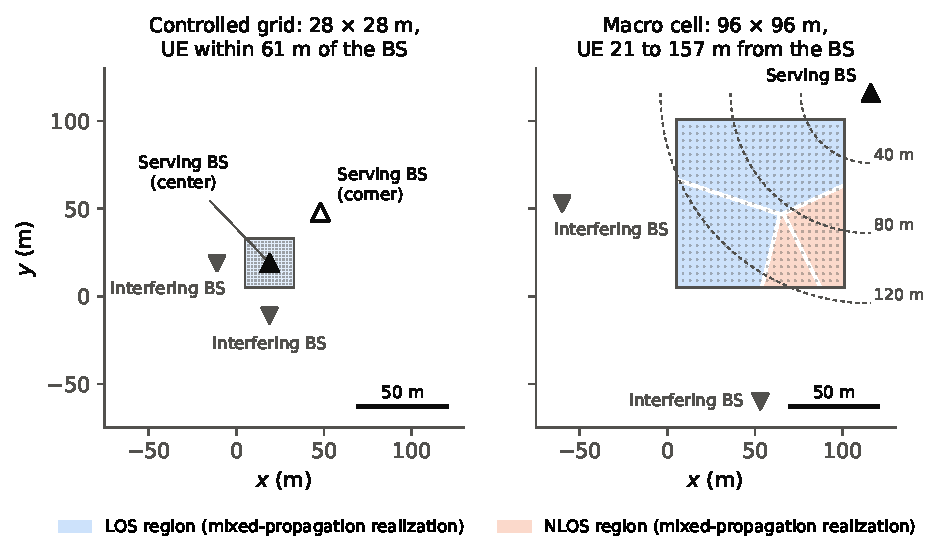
\includegraphics[width=0.95\textwidth]{fig_study_maps}
  \caption{The two deployments drawn at the same scale, with identical axes and a $50\,\text{m}$ scale bar in each panel. Left: the controlled grid, $15\times15$ cells at $2\,\text{m}$ pitch, with its two serving-BS placements~(filled: center; open: corner) and two interfering BSs. Right: the macro cell, $25\times25$ cells at $4\,\text{m}$ pitch, with the serving BS beyond its north-east corner, two interfering BSs, and range from the serving BS at $40$, $80$ and $120\,\text{m}$. Shading marks the macro cell's four Voronoi regions, park to the north and highway to the south-west~(LOS), shopping district to the south-east and residential area to the south~(NLOS), with the propagation each receives in the mixed-propagation realization; in the primary realization every region shares the same NLOS profile.}
  \label{fig:layout}
\end{figure}
% src: figure_scripts/make_figures.py study_maps(); grids, BS positions and Voronoi centres from the 15x15 and 25x25 configs; macro-cell transmitters from runners/run_multi_user_300_25x25.m (the 25x25 config's interferer entries, [-25,53] and [53,-25], are not used by that runner)

% src: configs/b6_los_blocked_los_config.jsonc (corridor length 200 m; strip widths 5-150 m; speeds 1.5, 4.0, 10.0 m/s; BS [100,500,10]; UMi LOS / UMi NLOS); CONTINUE_HERE.md §4 (360 users, constant-range rationale)
A fourth, targeted deployment, the \emph{blocked line-of-sight scenario}, follows UEs walking a straight $200\,\text{m}$ corridor whose middle section passes behind an obstruction, so that the link goes from LOS to NLOS and back. The width of the blocked strip is varied from $5$ to $150\,\text{m}$ and UE speed takes values of $1.5$, $4$ and $10\,\text{m/s}$. The BS stands $500\,\text{m}$ from the corridor so that range is nearly constant along it, which keeps the change in propagation from being confounded with a change in distance.

\subsection{Mobility}
\label{subsec:mobility}

% src: FINAL_REPORT.md §4.3
The controlled-grid study moves each UE on a random walk over the $8$-connected grid graph at $1.5\,\text{m/s}$; the walk carries no persistent heading. In the macro-cell study each user follows one of four trajectory patterns: straight-line navigation that reflects off the area boundary~($35\%$ of users), a random walk that continues straight with probability $0.7$~($35\%$), a tour between five sampled waypoints~($20\%$), or a straight transit across the area~($10\%$). Each user also belongs to one of four speed classes: pedestrian, $1.0$--$1.5\,\text{m/s}$~($40\%$); jogger, $2.5$--$4.5\,\text{m/s}$~($25\%$); vehicle, $8$--$15\,\text{m/s}$~($25\%$); or near-static, $0.1$--$0.5\,\text{m/s}$~($10\%$). All four patterns carry heading persistence, so the macro-cell mobility is favorable to history rather than adversarial to it.

% src: FINAL_REPORT.md §4.3, §5.8 (every step advances exactly one grid cell)
In both studies every step of a walk advances exactly one grid cell, and the time between snapshots is the step length divided by the UE's speed. A fixed history depth is therefore a fixed distance travelled, $h$ grid steps, but not a fixed duration: across the $232$ retained macro-cell users the time between snapshots $\Delta t$ ranges from $0.27$ to $32.5\,\text{s}$, with a median of $2.71\,\text{s}$. Position jitter of $\pm0.1\,\text{m}$ is added to every snapshot so that no estimator can latch onto exactly repeated coordinates.

\subsection{Device Model and AoA Impairment}
\label{subsec:device-model}

% src: FINAL_REPORT.md §4.4; technical_documentation.md §3.6, §3.7
The controlled-grid study simulates five device profiles: two four-antenna devices that differ only in their walk, a two-antenna device, a one-antenna device, and a two-antenna device carried at $0.9\,\text{m}$ height. The macro-cell study draws from a 3GPP-representative population of $85\%$ multi-antenna devices~(about $45\%$ with four antennas and $40\%$ with two) and $15\%$ single-antenna devices, each with its own antenna gain and carrying height. %TODO-CITE: 3GPP device-population mix assumption
Antenna count enters the channel through Equation~(\ref{eq:mrc}); the AoA capability of a device is then imposed when features are built, so the two device groups share an identical channel model and differ only in whether an angle is reported.

% src: FINAL_REPORT.md §4.4 (SINR-dependent model, controlled grid); csi_dataset.py load_and_prepare_data (macro cell: 4 deg Gaussian, 5 deg quantization, AoA = 0 for single-antenna devices)
Clean simulated arrival angles are degraded before use. In the controlled-grid study the noise on each axis depends on SINR,
\begin{equation}
  \sigma_{\text{AoA}}(t) = \operatorname{clamp}\!\left(2.0^\circ \cdot 10^{-\frac{\mathrm{SINR}_{dB}(t)-10}{15}},\ 1.0^\circ,\ 20.0^\circ\right),
  \label{eq:aoa-noise}
\end{equation}
while the macro-cell study applies a fixed $4^\circ$ Gaussian error, drawn independently for every report, an assumption that Section~\ref{subsec:averaging} shows to matter. Both then quantize azimuth and elevation to a $5^\circ$ codebook. Single-antenna devices cannot form a beam and report no angle; in the macro-cell features their angle is set to $0^\circ$.

\subsection{Features}
\label{subsec:features}

% src: technical_documentation.md §4.1-4.3
In the controlled-grid study, $\mathbf{m}(t)$ contains RSS and SINR, optionally extended with the AoA pair and with three device parameters: antenna count, antenna gain, and carrying height. The window of Equation~(\ref{eq:transition-history}) is built per user after sorting by time; the first $h$ snapshots of each user are dropped, and no window crosses from one user to another. Values are stacked in absolute form, because device-specific RSS and SINR offsets are stable across the grid and themselves act as fingerprints.

% src: FINAL_REPORT.md §4.5; csi_dataset.py build_derived_features (d_rss, d_az, d_ray_x, d_ray_y are per-user first differences divided by delta_t; ray = FSPL range estimate x AoA unit vector)
In the macro-cell study, each snapshot carries $13$ channels: RSS, SINR, the sines and cosines of both angles, which remove the $\pm180^\circ$ wrap discontinuity, two ray-projection coordinates formed from a path-loss range estimate and the AoA unit vector, the time increment $\Delta t$, and first differences of RSS, azimuth, and the two ray coordinates with respect to the previous snapshot, each divided by $\Delta t$. Every derived channel is computable from the raw measurements, so the derived set adds inductive bias rather than information. Because the first differences are part of each snapshot, the $h=0$ input of the macro-cell study already contains one step of change; it is the current snapshot together with its difference from the previous one, and the $h=5$ input stacks six such snapshots. Three static device features, antenna count, antenna gain, and carrying height, accompany every input.

\subsection{Estimators}
\label{subsec:estimators}

% src: CSI-Location experiments_ablation/model_zoo.py (build_classical, build_net, training constants); master_benchmark_rerun_summary.json (n_params)
The macro-cell study evaluates seven estimators spanning five algorithmic paradigms, listed in Table~\ref{tab:estimators}: $k$-nearest neighbors~($k$-NN), Random Forest, XGBoost, a gated recurrent unit~(GRU) network, and three one-dimensional convolutional neural networks~(1D-CNN), one with an AoA-validity channel and one with temporal self-attention. Hyperparameters are held fixed across history depths, so the input window is the only factor that varies within a model. The four neural models share a training recipe, AdamW at a learning rate of $3\times10^{-4}$ with weight decay $10^{-2}$, batch size $512$, a Huber loss on position with auxiliary speed and uncertainty heads, and at most $60$ epochs with early stopping. The controlled-grid study uses Random Forest and XGBoost classifiers, and its grid-size sweep adds a Gaussian likelihood model and a multilayer perceptron.

\begin{table}[h]
  \centering
  \caption{Estimators used in the macro-cell study.}
  \label{tab:estimators}
  \small
  \begin{tabular}{@{}lll@{}}
    \toprule
    Paradigm & Model & Configuration \\
    \midrule
    Instance-based & $k$-NN & $k=5$ \\
    Bagged trees & Random Forest & 150 trees, depth 16, min.\ leaf 5 \\
    Boosted trees & XGBoost & 50 trees, depth 5, learning rate 0.15 \\
    Recurrent & GRU & 2 layers, 254\,K parameters \\
    Convolutional & 1D-CNN & 3 convolutional layers, 67\,K parameters \\
    Convolutional & Mask-aware 1D-CNN & 1D-CNN with an AoA-validity channel, 67\,K parameters \\
    Attention & 1D-CNN with temporal self-attention & 200\,K parameters \\
    \bottomrule
  \end{tabular}
\end{table}

\subsection{Evaluation Protocol}
\label{subsec:protocol}

% src: FINAL_REPORT.md §4.7
The controlled-grid study splits each user's walk in time, training on the first $80\%$ of steps and testing on the last $20\%$; a random split would leak, because spatial consistency makes temporally adjacent samples near-duplicates. It is scored by exact-cell accuracy. The macro-cell study splits over users, so that the $47$ test users of each split are never seen during training, and it is scored by the 2D Euclidean error between predicted and true position: its mean, median, and 90th percentile, and the fraction of predictions within $5$, $10$ and $20\,\text{m}$. Every macro-cell result is reported separately for multi-antenna and single-antenna devices.

% src: seed_repeats_all_models.py docstring (seed drives split and init; marginal vs seed-paired)
The primary comparison is the change in error when history is added, measured within one model against its own $h=0$ input. For the macro-cell headline results the whole protocol is repeated over five seeds, each of which draws a different user split and model initialization. Two uncertainties follow. The marginal spread across seeds measures how much a single reported number could move by chance, and it is dominated by which users happen to land in the test set. The seed-paired difference compares two inputs on the same split and so cancels that source; it is the appropriate test for a change of input, and its $95\%$ confidence interval is reported with each gain.

% src: experiments_ablation/model_zoo.py train_deep docstring (early stopping on test MAE)
The neural models select their stopping epoch by error on the test users. This applies equally to both depths of a model, so within-model comparisons are unaffected, but it makes the absolute errors of the neural models, and any comparison between a neural model and a tree or instance-based model, optimistic in the neural model's favor.
